\chapter{Uniones}

\section{Elección del Método de Unión}
El Perfil se fabricará en acero, por tanto se nos presentan dos vías posibles para realizar la unión:
\begin{itemize}
    \item Soldadura. Bien sea por puntos o la oxiacetilénica.
    \item Remachado.
\end{itemize}

En general, la elección del método de unión dependerá de consideraciones sobre la eficiencia, costo y otros factores. En este caso, al ser un perfil aerodinámico, necesitamos evitar a toda costa cualquier tipo de deformación, pues estas, por pequeñas que sean, podrían afectar a la aerodinámica e invalidar el ensayo. Por ende, descartamos la soldadura, que genera deformaciones inherentemente, en favor del remachado.

\subsection{Elección del Remachado}
La elección del tipo de remachado dependerá de diversos factores: tipo de unión, accesibilidad, ubicación, etc. Según su accesibilidad, se nos presentan dos opciones:
\begin{itemize}
    \item Remaches de caña maciza. Permiten el acceso por ambos lados de la unión, y proporcionan mayor resistencia. 
    \item Remaches ciegos. Tan solo permite el acceso por un lado de la unión.
\end{itemize}

Por tanto, basándonos en lo anterior, elegiremos remaches de cabeza avellanada en zonas con requerimientos aerodinámicos, pero optaremos por remaches de cabeza universal\footnote{También conocidos como de \textit{gota de sebo}.} en zonas sin estos requerimientos, por ser más económicos. Cuando haya accesibilidad por sendos lados, optaremos por usar remaches de caña maciza, por ser más resistentes. En todos los casos, los remaches serán de cabeza normal, lo que asegura tanto la calidad como la funcionalidad de las uniones.

\section{Cálculo de los Remaches}

Basándonos en la normativa aplicable, para un remache de cabeza de cierre normal, se usan las siguientes expresiones:
\begin{gather}
    l = e + 1.5d, \\
    D = 1.5d, \\
    K = 0.4d,
\end{gather}

donde $l$ es la longitud de la caña, $d,$ el diámetro del remache, $D$ el diámetro de la cabeza de cierre, y $K$ la longitud de la cabeza del remache (ver figura \ref{fig:remaches}).
\begin{figure}[!htb]
    \centering
    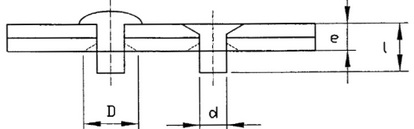
\includegraphics[width=0.5\linewidth]{Figures/remaches.png}
    \caption{Representación de medidas de un remache de cabeza normal y de un remache avellanado}
    \label{fig:remaches}
\end{figure}

En el caso de remaches con cabeza avellanada, empleamos:
\begin{gather}
    l = e_T + 0.8d = 5.2 \quad \text{[mm]}, \\
    D = 2d = 8 \quad \text{[mm]}, \\
\end{gather}

siendo $e_T$ el espesor total de la chapas a unir. 

Según \textit{Remaches y Herramientas}\cite{remaches} y considerando acero, $d = 4 \text{[mm]}$ para los remaches, y un espesor de la chapa de $e_{\text{Ac}} = 1 \text{[mm]}$.

Se ha elegido una distancia al borde del remache de $10 \text{[mm]}$, que es $0.5 \text{[mm]}$ más que la distancia mínima recomendada por la normativa:
\begin{equation}
    E \ge 2d + 1.5 = 9.5 \quad \text{[mm]}.
\end{equation}

Respecto a la distancia entre remaches, la normativa marca que debe ser, al menos, cuatro veces el diámetro para remaches (ver figura \ref{fig:dist}):

\begin{equation} \label{eq:p}
    P > 4d = 16 \quad \text{[mm]}.
\end{equation}

\begin{figure}[!htb]
    \centering
    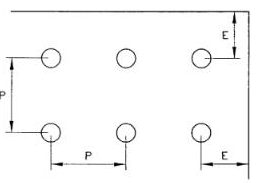
\includegraphics[width=0.3\linewidth]{Figures/distancia.png}
    \caption{Distancia entre remaches}
    \label{fig:dist}
\end{figure}

Las uniones quedan recogidas a continuación\footnote{Cálculos redondeados a la baja}:

\begin{table}[!htb]\centering

\begin{tabular}{|l|r|}\hline
\rowcolor[HTML]{C0C0C0}\textbf{Línea de Unión} 
& \textbf{Tipo de Soldadura}\\\hline
Sombreretes - Tubo & Soldadura oxiacetilénica \\\hline
Larguerillo - Costilla & Soldadura por puntos \\\hline
\end{tabular}
\end{table}

\begin{landscape}
    \vspace*{\fill}
    \begin{table}[H]\centering

\begin{tabular}{|l|r|r|r|}\hline
\rowcolor[HTML]{C0C0C0}\textbf{Línea de Unión} &\textbf{Tipo de Caña} &\textbf{Cabeza} &\textbf{Longitud \tablefootnote{Longitud sin Deformar} [mm]} \\\hline
Unión Sombrerete - Costilla &Caña maciza &Universal &8 \\\hline
Revestimiento borde de ataque – Costilla ($\times 3$) &Ciego y caña maciza &Universal &8 \\\hline
Zona plana revestimiento del borde de salida ($\times 3$) &Ciego &Avellanada \tablefootnote{Zona con función aerodinámica, por tanto se ha de usar remachado avellanado. Se calcula usando cabezas de tipo universal para facilitar los cálculos. \label{av}}  &8 \\\hline
Zona curva revestimiento del borde de salida ($\times 3$) &Ciego &Avellanada \footref{av}  &8 \\\hline
Revestimiento borde de ataque – Revestimiento extradós  ($\times 3$) &Caña maciza &Avellanada &8 \\\hline
Revestimiento borde de ataque – Revestimiento intradós ($\times 3$) &Ciego &Avellanada \footref{av} &8 \\\hline
Revestimiento borde de salida – Revestimiento intradós  ($\times 3$)&Ciego &Avellanada \footref{av} &8 \\\hline
Revestimiento extradós ($\times 3$)&Caña maciza &Avellanada \footref{av} &8 \\\hline
Revestimiento intradós  ($\times 3$) &Caña maciza &Avellanada &8 \\\hline
Revestimiento borde de salida – Revestimiento extradós  ($\times 3$) &Caña maciza &Avellanada \footref{av} &8 \\\hline
Larguerillo delantero – Revestimiento intradós &Ciego &Avellanada \footref{av} &8 \\\hline
Larguerillo delantero – Revestimiento extradós &Caña maciza &Avellanada \footref{av} &8 \\\hline
Larguerillo trasero – Revestimiento borde de salida &Ciego &Avellanada \footref{av} &8 \\\hline
Tapa acceso - Costilla exterior ($\times 2$) &Caña maciza &Avellanado &8 \\ \hline
\end{tabular}
\end{table}
    \vspace*{\fill}
    \clearpage
\end{landscape}

\subsection{Cálculos Uniones}
\subsubsection{Unión Sombretes - Costillas}
Empleamos remaches de caña maciza y cabeza normal (por cuestión de accesibilidad) equiespaciados entre sí 17 [mm], superior a la distancia dada por la ecuación \ref{eq:p}. El remachado se hace a lo largo de la línea media. Al existir tres costillas con un sombrerete cada una, necesitaremos un total de 96 remaches.

\begin{equation}
    L_s = 2\pi \bigg( \dfrac{200-162}{2} + \dfrac{162}{2} \bigg) = 568.63 \quad \text{[mm]}.
\end{equation}

Al haber un acceso, tendremos que restar 20 [mm] al perímetro de la línea media:
\begin{equation}
    L_{s,\, \text{real}} = 548.63 \quad \text{[mm]}.
\end{equation}

El número de remaches se calcula como:
\begin{equation}
    N = \dfrac{548.63}{17} = 32.27 \approx 32 \quad \text{[Remaches]} \times \text{Costilla}.
\end{equation}

La distancia real es:
\begin{equation}
    P_{\text{real}} = \dfrac{548.63}{32} = 17.15 \quad \text{[mm]}
\end{equation}

\subsubsection{Revestimiento Borde de Ataque - Costillas} \label{subsub:ba}
Vamos a necesitar taladrar los puntos donde se vayan a utilizar remaches. El bordonado no se taladrará ni remachará aún\footnote{Se hará cuando se instalen los revestimientos del extradós e intradós, para asegurar la alineación}, pero se tendrá en cuenta para el cálculo. Estos agujeros atravesarán los dos revestimientos y la costilla sin presentar desviaciones.

Todos los remaches se situarán en la línea media de la solapa, y se tendrá en cuenta 9.5 [mm] de espaciado hasta los bordes.

Unión de revestimiento del borde de ataque - costillas:
\begin{equation}
    L_r = 1099.32 \quad \text{[mm]}.
\end{equation}

Longitud real del remachadao, teniendo en cuenta los espaciados desde los bordes:
\begin{equation}
    L_{\text{real}} = 1099.32 - 2 \cdot 10 = 1079.32 \quad \text{[mm]}.
\end{equation}

Número de remaches:
\begin{equation}
    N = \dfrac{1079.32}{17} = 63.49 \approx 63 \quad \text{Remaches} \times \text{Costilla}.
\end{equation}

\begin{equation}
    P_{\text{real}} = \dfrac{1079.32}{63} = 17.13 \quad \text{[mm]}
\end{equation}

Dejaremos los remaches de los bordes sin remachar, por tanto, el número de remaches utilizados serán 2 menos por costilla, por lo que habrá un total de 183 remaches hasta el bordonado.

\subsubsection{Unión Larguerillos - Costillas}
Se debe proceder con cuidado para asegurar una unión adecuada sin comprometer la integridad estructural o la aerodinámica de la pieza. Usaremos la soldadura por puntos, empleando un equipo de soldadura por resistencia, que es muy efectiva para reducir la deformación del material, puesto que el calor se concentra solo en los puntos de soldadura, reduciendo el efecto térmico.

\subsubsection{Revestimiento Borde de Salida - Costillas} \label{subsub:bs}
Mismo procedimiento que el explicado en \ref{subsub:ba}. Los remaches se colocan en la línea media de la solapa de las costillas en contacto con el revestimiento, dejando un espaciado de 10 [mm] a los bordes.

Unión revestimiento:
\begin{equation}
    L_r = 602.4 \quad \text{[mm]}.
\end{equation}

Longitud real del remachado:
\begin{equation}
    L_{\text{real}} = 602.4 - 2 \times 10 = 584.4 \quad \text{[mm]}.
\end{equation}

Número de remaches:
\begin{equation}
    N = \dfrac{584.4}{17} = 34.38 \approx 34 \quad \text{Remaches} \times \text{Costilla}.
\end{equation}

\begin{equation}
    P_{\text{real}} = \dfrac{584.4}{34} = 17.19 \quad \text{[mm]}
\end{equation}

Al igual que pasaba en \ref{subsub:ba}, el número de remaches es 2 menos por costilla. Es decir, hay un total de 102 remaches hasta el bordonado.

\subsubsection{Revestimiento Borde de Ataque - Revestimiento Extra e Intradós} \label{subsub:rba}
En el primer bordonado comienza el revestimiento del extradós e intradós, por lo que habrá un remache justo en el centro del bordonado, dejando 10 [mm] hasta el borde. Es decir, habrá que poner los remaches que no hemos puesto en \ref{subsub:ba}.


\subsubsection{Revestimiento Borde de Salida - Revestimiento Extra e Intradós}
Procedemos análogamente a \ref{subsub:rba}. Teniendo en cuenta lo expuesto en \ref{subsub:bs}, tendremos que colocar los 6 remaches que no pusimos entonces.

\subsubsection{Larguerillos - Revestimiento Extradós e Intadós}
Por cada larguerillo habrá dos hileras de remaches separadas entre sí por 20 [mm] y que se sitúan entre las dos costillas exteriores\footnote{Recordemos que estarán unidas por soldadura por punto}. Las dos hileras se encargan de unir el revestimiento en cuestión al larguerillo. 

Como la longitud entre costillas es de 400 [mm]:
\begin{equation}
    L_r = (400 - 4 \cdot 10) = 360 \quad \text{[mm] $\times$ larguerillo}.
\end{equation}

Número de remaches:
\begin{equation}
    N = \dfrac{360}{17} = 21.18 \approx 21 \quad \text{Remaches}.
\end{equation}

\begin{equation}
    P_{\text{real}} = \dfrac{360}{21} = 17.14 \quad \text{[mm]}.
\end{equation}

\subsubsection{Tapa de Acceso - Solapes de Acceso - Costilla}
La costilla proporciona dos solapes a cada lado del acceso, que van unidos a la propia costilla mediante una hilera de remaches. Posteriormente, al otro lado del solape que sobrasale 20 [mm] en la apertura de acceso, se remachará en la línea media con la tapa, dejando, para ambos casos, 10 [mm] en los bordes\footnote{Cumple lo establecido en la normativa, 9.5 [mm]}, ya que el solape mide 40 [mm].

\begin{equation}
    L_r = 180 - 2 \cdot 10 = 160 \quad \text{[mm]}.
\end{equation}

Número de remaches:
\begin{equation}
    N = \dfrac{160}{17} = 9.41 \approx 9 \quad \text{Remaches $\times$ Hilera}.
\end{equation}

Espaciado entre remaches:
\begin{equation}
    P_{\text{real}} = \dfrac{160}{9} = 177.78 \quad \text{[mm]}.
\end{equation}

\subsubsection{Revestimiento Intradós - Costilla}

\begin{equation}
    L_r = 426.29 - 2 \cdot 10 = 406.29 \quad \text{[mm]}.
\end{equation}

Número de remaches:
\begin{equation}
    N = \dfrac{406.29}{17} = 23.90 \approx 23 \quad \text{Remaches $\times$ Costilla}.
\end{equation}

Espaciado entre remaches:
\begin{equation}
    P_{\text{real}} = \dfrac{406.29}{23} = 17.66 \quad \text{[mm]}.
\end{equation}

\subsubsection{Revestimiento Extradós - Costilla}
\begin{equation}
    L_r = 320 - 2 \times 10 = 300 \quad \text{[mm]} 
\end{equation}

Número de remaches:
\begin{equation}
    N = \dfrac{300}{17} = 17.65 \approx 17 \quad \text{Remaches $\times$ Costilla}.
\end{equation}

Espaciado entre remaches:
\begin{equation}
    P_{\text{real}} = \dfrac{300}{17} = 17.65 \quad \text{[mm]}
\end{equation}

\subsubsection{Soldadura Tubo - Sombreretes}
Decidimos soldar el tubo y los sombreretes mediante soldadura oxiacetilénica. Al fundirse el límite entre ambas piezas, no se discernirá que son piezas diferentes.

Los Autores aclaramos que, a pesar de que sí que habrá una zona afectada por el calor (i.e. con deformación), no afectará a la aerodinámica.